\documentclass{article}
\usepackage[utf8]{inputenc}
\usepackage{hyperref}
\usepackage[letterpaper, portrait, margin=1in]{geometry}
\usepackage{enumitem}
\usepackage{amsmath}
\usepackage{booktabs}
\usepackage{graphicx}

\usepackage{hyperref}
\hypersetup{
colorlinks=true,
    linkcolor=black,
    filecolor=black,      
    urlcolor=blue,
    citecolor=black,
}
\usepackage{natbib}

\usepackage{titlesec}
  
\title{Homework 3}
\author{Ryan Ellis}
\date{Spring semester 2023}
  
\begin{document}
  
\maketitle

\section{Part 1: Math}

\subsection{A}
The following steps prove the equality by the properties of logarithms:

\begin{align}
    y_i &= e^\alpha \delta^{d_i} z^\gamma_i e^{\eta_i}
\end{align}

\begin{align}
    ln{(y_i)} = ln{(e^\alpha \delta^{d_i} z^\gamma_i e^{\eta_i})}
\end{align}

\begin{align}
    = ln{(e^\alpha)} + ln{(\delta^{d_i})} + ln{(z^\gamma_i)} + ln{(e^{\eta_i})}
\end{align}

\begin{align}
    = \alpha + ln{(\delta^{d_i})} + ln{(z^\gamma_i)} + \eta_i
\end{align}

\begin{align}
    = \alpha + ln{(\delta)}d_i + \gamma ln{(z_i)} + \eta_i
\end{align}

\subsection{B}

The parameter $\delta$ is a multiplicative \textbf{factor representing the retrofit's effect on energy production}.

\subsection{C}

We want to show proof of the following equality:

\begin{align}
    \frac{\Delta y_i}{\Delta {d_i}}  = \frac{\delta - 1}{\delta ^ {d_i}} y_i
\end{align}

Since coefficient $\delta$ is only "activated" by the binary variable $d_i$ taking a value of 1, we can think of the following expression with potential outcomes notation,

\begin{align}
    y_i (\delta - 1) = \delta y_i - y_i = y_{1i} - y_{0i} = \Delta y_i
\end{align}

If the above (8) is the numerator of equation (7), we can use the same notation to rework the denominator too:

\begin{align}
    \delta^{d_i} = d_1i - d_0i = \Delta d_i
\end{align}

Combining (8) and (9) gives us the original equality,

\begin{align}
    \frac{\Delta y_i}{\Delta {d_i}}  = \frac{\delta - 1}{\delta ^ {d_i}} y_i
\end{align}

This term is the \textbf{average marginal effect} of $d_i$.

\subsection{D}

We want to show that the following equality holds:

\begin{align}
    \frac{\partial y_i}{\partial z_i} = \gamma \frac{y_i}{z_i}
\end{align}

Using properties of exponents and partial derivatives, we manipulate terms.

\begin{align}
    \frac{\partial y_i}{\partial z_i} \left(e^\alpha \delta^{d_i} z^\gamma_i e^{\eta_i}\right) = \gamma z_i ^ {\gamma - 1} \left(e^\alpha \delta^{d_i}e^{\eta_i}\right)
\end{align}

\begin{align}
    = \gamma z_i ^{\gamma - 1} \left(\frac{y_i}{z_i^\gamma} \right)
\end{align}

\begin{align}
    = \gamma \left[\frac{y_i (z_i ^{\gamma - 1})}{z_i^\gamma} \right]
\end{align}

\begin{align}
    = \gamma \left[y_i \left(z_i ^ {\gamma - 1 - \gamma} \right) \right]
\end{align}

\begin{align}
    = \gamma y_i z_i ^{-1} \hspace{2cm}= \gamma \frac{y_i}{z_i}
\end{align}

This term is the \textbf{average marginal effect} of $z_i$.


\vspace{10cm}
\section{Part 2: Stata}

\subsection{Estimation}


\documentclass{article}
\usepackage{multirow}
\usepackage{amsmath}
\usepackage{ulem}
\usepackage[table]{xcolor}
\begin{document}
\begin{table}[!h]
\caption{Regression results and Marginal Effects}
\centering
\begin{tabular}{lll}
\cline{1-3}
\multicolumn{1}{r}{} &
  \multicolumn{1}{c}{1} &
  \multicolumn{1}{c}{2} \\
\cline{1-3}
\multicolumn{1}{l}{Retrofit} &
  \multicolumn{1}{c}{-0.101} &
  \multicolumn{1}{c}{} \\
\multicolumn{1}{l}{} &
  \multicolumn{1}{c}{[-0.113    -0.088]} &
  \multicolumn{1}{c}{} \\
\multicolumn{1}{l}{ln(Square Feet)} &
  \multicolumn{1}{c}{0.894} &
  \multicolumn{1}{c}{} \\
\multicolumn{1}{l}{} &
  \multicolumn{1}{c}{[0.880     0.909]} &
  \multicolumn{1}{c}{} \\
\multicolumn{1}{l}{ln(Temperature (F))} &
  \multicolumn{1}{c}{0.281} &
  \multicolumn{1}{c}{} \\
\multicolumn{1}{l}{} &
  \multicolumn{1}{c}{[0.040     0.523]} &
  \multicolumn{1}{c}{} \\
\multicolumn{1}{l}{Intercept} &
  \multicolumn{1}{c}{-0.769} &
  \multicolumn{1}{c}{} \\
\multicolumn{1}{l}{} &
  \multicolumn{1}{c}{[-1.834     0.296]} &
  \multicolumn{1}{c}{} \\
\multicolumn{1}{l}{Marginal Effects, Retrofit} &
  \multicolumn{1}{c}{} &
  \multicolumn{1}{c}{-114.050} \\
\multicolumn{1}{l}{} &
  \multicolumn{1}{c}{} &
  \multicolumn{1}{c}{[-114.521  -113.578]} \\
\multicolumn{1}{l}{Marginal Effects, Square Feet} &
  \multicolumn{1}{c}{} &
  \multicolumn{1}{c}{0.629} \\
\multicolumn{1}{l}{} &
  \multicolumn{1}{c}{} &
  \multicolumn{1}{c}{[0.628     0.629]} \\
\multicolumn{1}{l}{Marginal Effects, Temperature (F)} &
  \multicolumn{1}{c}{} &
  \multicolumn{1}{c}{4.077} \\
\multicolumn{1}{l}{} &
  \multicolumn{1}{c}{} &
  \multicolumn{1}{c}{[3.969     4.185]} \\
\multicolumn{1}{l}{Number of observations} &
  \multicolumn{1}{c}{1000} &
  \multicolumn{1}{c}{1000} \\
\cline{1-3}
\end{tabular}
\end{table}
\end{document}


\vspace{1cm}
\subsection{Graph}

\begin{figure}[ht]
    \centering
    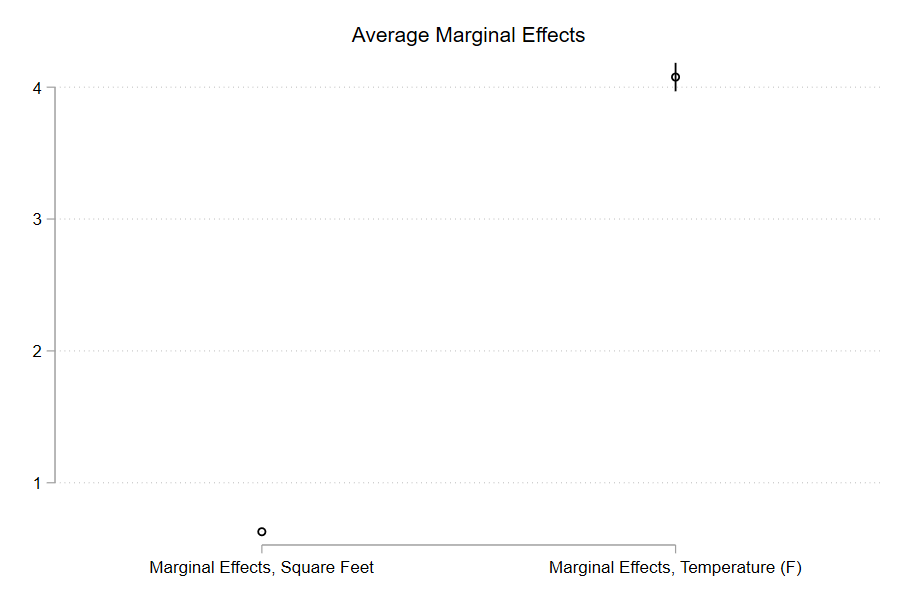
\includegraphics[scale = 0.4]{homework3/output/ame_hw3.png}
\end{figure}

\end{document}